% !TEX root = ../main.tex

\section{Model development}

This section presents the equations used to convert the measured data to different bases for use in the reactor models. The biomass pyrolysis kinetics scheme along with the associated biomass characterization method is also detailed. Finally, the reduced-order batch and continous stirred tank reactor (CSTR) models are presented.

\subsection{Basis of analysis}

The proximate analysis data is converted to different bases using ASTM methods \cite{Astm-2015}. Equations \ref{eq:prox-bases1}--\ref{eq:prox-bases4} convert the as-determined (AD) basis to as-received (AR), dry (D), and dry ash-free (DAF) bases where $P$ is the wt. \% of the corresponding basis parameter, $M$ is the moisture content, and $ADL$ is the air-dry loss assumed to be 22 wt. \%. As an example, to obtain the as-received value of the fixed carbon use $FC_{ar} = FC_{ad} \times \frac{100 - M_{ar}}{100 - M_{ad}}$.

\begin{align}
    M_{ar} &= \left(M_{ad} \times \frac{100 - ADL}{100}\right) + ADL \label{eq:prox-bases1} \\
    P_{ar} &= P_{ad} \times \frac{100 - M_{ar}}{100 - M_{ad}} \\
    P_{d} &= P_{ad} \times \frac{100}{100 - M_{ad}} \\
    P_{daf} &= P_{ad} \times \frac{100}{100 - M_{ad} - ash_{ad}} \label{eq:prox-bases4}
\end{align}

Similarly, the ultimate analysis data is also converted to different bases using the ASTM methods \cite{Astm-2015}. Equations \ref{eq:prox-bases1}--\ref{eq:prox-bases4} convert the carbon, nitrogen, and sulfur fractions to different bases while Equations \ref{eq:ult-bases1}--\ref{eq:ult-bases4} are for the hydrogen and oxygen fractions. Equation \ref{eq:cho-basis} calculates the CHO basis from the dry ash-free basis.

\begin{align}
    H_{ar} &= (H_{ad} - 0.1119\, M_{ad}) \times \frac{100 - M_{ar}}{100 - M_{ad}} \label{eq:ult-bases1} \\
    O_{ar} &= (O_{ad} - 0.8881\, M_{ad}) \times \frac{100 - M_{ar}}{100 - M_{ad}} \\
    H_{d} &= (H_{ad} - 0.1119\, M_{ad}) \times \frac{100}{100 - M_{ad}} \\
    O_{d} &= (O_{ad} - 0.8881\, M_{ad}) \times \frac{100}{100 - M_{ad}} \label{eq:ult-bases4} \\
    P_{cho} &= P_{daf} \times \frac{100}{100 - N_{daf} - S_{daf}} \label{eq:cho-basis}
\end{align}

For the chemical analysis data, the given dry basis values $P_d$ are converted to a dry ash-free basis $P_{daf}$ using Equation \ref{eq:chem-daf} where $P_{struct}$ is the structural inorganics, $P_{nonstruct}$ is the non-structural inorganics, and $P_{d,\,total}$ is the sum of the dry basis values.

\begin{equation}
    \label{eq:chem-daf}
    P_{daf} = P_d \times \frac{100}{P_{d,\,total} - P_{struct} - P_{nonstruct}}
\end{equation}

\subsection{Biomass pyrolysis kinetics}

The kinetic reaction mechanisms presented in the Debiagi et al. 2018 paper \cite{Debiagi-2018} are used to model biomass pyrolysis in the fluidized bed reactor. Table \ref{tab:chem-kinetics} summarizes the reactions along with the associated prefactors and activation energies. A description of the chemical species in the Debiagi et al. kinetic scheme is provided in Table \ref{tab:chem-species}.

% \setlength\LTleft{-0.2in}
% \setlength\LTright{-0.2in}
\begin{center}
\footnotesize
\begin{longtable}{cp{4in}rr}
    \caption{Kinetic reactions for biomass pyrolysis where A is the prefactor, E is the activation energy, and T is temperature. Source \cite{Debiagi-2018}.}
    \label{tab:chem-kinetics} \\
    \toprule
    Item & Reaction & A (1/s) & E (cal/mol) \\
    \midrule
    1  & CELL $\rightarrow$ CELLA & 1.5 $\times$ 10$^{14}$ & 47,000 \\
    2  & CELLA $\rightarrow$ 0.40 CH2OHCHO + 0.03 CHOCHO + 0.17 CH3CHO + 0.25 C6H6O3 + 0.35 C2H5CHO + 0.20 CH3OH + 0.15 CH2O + 0.49 CO + 0.05 G\{CO\} + 0.43 CO2 + 0.13 H2 + 0.93 H2O + 0.05 G\{COH2\} loose + 0.02 HCOOH + 0.05 CH2OHCH2CHO + 0.05 CH4 + 0.1 G\{H2\} + 0.66 CHAR & 2.5 $\times$ 10$^6$ & 19,100 \\
    3  & CELLA $\rightarrow$ C6H10O5 & 3.3 $\times$ T & 10,000 \\
    4  & CELL $\rightarrow$ 4.45 H2O + 5.45 CHAR + 0.12 G\{COH2\} stiff + 0.18 G\{COH2\} loose + 0.25 G\{CO\} + 0.125 G\{H2\} + 0.125 H2 & 9.0 $\times$ 10$^7$ & 31,000 \\
    5  & GMSW $\rightarrow$ 0.70 HCE1 + 0.30 HCE2 & 1.0 $\times$ 10$^{10}$ & 31,000 \\
    6  & XYHW $\rightarrow$ 0.35 HCE1 + 0.65 HCE2 & 1.25 $\times$ 10$^{11}$ & 31,400 \\
    7  & XYGR $\rightarrow$ 0.12 HCE1 + 0.88 HCE2 & 1.25 $\times$ 10$^{11}$ & 30,000 \\
    8  & HCE1 $\rightarrow$ 0.25 C5H8O4 + 0.25 C6H10O5 + 0.16 FURFURAL + 0.13 C6H6O3 + 0.09 CO2 + 0.1 CH4 + 0.54 H2O + 0.06 CH2OHCH2CHO + 0.1 CHOCHO + 0.02 H2 + 0.1 CHAR & 16.0 $\times$ T & 12,900 \\
    9  & HCE1 $\rightarrow$ 0.4 H2O + 0.39 CO2 + 0.05 HCOOH + 0.49 CO + 0.01 G\{CO\} + 0.51 G\{CO2\} + 0.05 G\{H2\} + 0.4 CH2O + 0.43 G\{COH2\} loose + 0.3 CH4 + 0.325 G\{CH4\} + 0.1 C2H4 + 0.075 G\{C2H4\} + 0.975 CHAR + 0.37 G\{COH2\} stiff + 0.1 H2 + 0.2 G\{C2H6\} & 3.0 $\times$ 10$^{-3}$ $\times$ T & 3,600 \\
    10 & HCE2 $\rightarrow$ 0.3 CO + 0.5125 CO2 + 0.1895 CH4 + 0.5505 H2 + 0.056 H2O + 0.049 C2H5OH + 0.035 CH2OHCHO + 0.105 CH3CO2H + 0.0175 HCOOH + 0.145 FURFURAL + 0.05 G\{CH4\} + 0.105 G\{CH3OH\} + 0.1 G\{C2H4\} + 0.45 G\{CO2\} + 0.18 G\{COH2\} loose + 0.7125 CHAR + 0.21 G\{H2\} + 0.78 G\{COH2\} stiff + 0.2 G\{C2H6\} & 7.0 $\times$ 10$^9$ & 30,500 \\
    11 & LIGH $\rightarrow$ LIGOH + 0.5 C2H5CHO + 0.4 C2H4 + 0.2 CH2OHCHO + 0.1 CO + 0.1 C2H6 & 6.7 $\times$ 10$^{12}$ & 37,500 \\
    12 & LIGO $\rightarrow$ LIGOH + CO2 & 3.3 $\times$ 10$^8$ & 25,500 \\
    13 & LIGC $\rightarrow$ 0.35 LIGCC + 0.1 VANILLIN + 0.1 C6H5OCH3 + 0.27 C2H4 + H2O + 0.17 G\{COH2\} loose + 0.4 G\{COH2\} stiff + 0.22 CH2O + 0.21 CO + 0.1 CO2 + 0.36 G\{CH4\} + 5.85 CHAR + 0.2 G\{C2H6\} + 0.1 G\{H2\} & 1.0 $\times$ 10$^{11}$ & 37,200 \\
    14 & LIGCC $\rightarrow$ 0.25 VANILLIN + 0.15 CRESOL + 0.15 C6H5OCH3 + 0.35 CH2OHCHO + 0.7 H2O + 0.45 CH4 + 0.3 C2H4 + 0.7 H2 + 1.15 CO + 0.4 G\{CO\} + 6.80 CHAR + 0.4 C2H6 & 1.0 $\times$ 10$^4$ & 24,800 \\
    15 & LIGOH $\rightarrow$ 0.9 LIG + H2O + 0.1 CH4 + 0.6 CH3OH + 0.3 G\{CH3OH\} + 0.05 CO2 + 0.65 CO + 0.6 G\{CO\} + 0.05 HCOOH + 0.45 G\{COH2\} loose + 0.4 G\{COH2\} stiff + 0.25 G\{CH4\} + 0.1 G\{C2H4\} + 0.15 G\{C2H6\} + 4.25 CHAR + 0.025 C24H28O4 + 0.1 C2H3CHO & 1.5 $\times$ 10$^8$ & 30,000 \\
    16 & LIG $\rightarrow$ VANILLIN + 0.1 C6H5OCH3 + 0.5 C2H4 + 0.6 CO + 0.3 CH3CHO + 0.1 CHAR & 4.0 $\times$ T & 12,000 \\
    17 & LIG $\rightarrow$ 0.6 H2O + 0.3 CO + 0.1 CO2 + 0.2 CH4 + 0.4 CH2O + 0.2 G\{CO\} + 0.4 G\{CH4\} + 0.5 G\{C2H4\} + 0.4 G\{CH3OH\} + 1.25 G\{COH2\} loose + 0.65 G\{COH2\} stiff + 6.1 CHAR + 0.1 G\{H2\} & 8.3 $\times$ 10$^{-2}$ $\times$ T & 8,000 \\
    18 & LIG $\rightarrow$ 0.6 H2O + 2.6 CO + 0.6 CH4 + 0.4 CH2O + 0.75 C2H4 + 0.4 CH3OH + 4.5 CHAR + 0.5 C2H6 & 1.5 $\times$ 10$^9$ & 31,500 \\
    19 & TGL $\rightarrow$ C2H3CHO + 2.5 MLINO + 0.5 U2ME12 & 7.0 $\times$ 10$^{12}$ & 45,700 \\
    20 & TANN $\rightarrow$ 0.85 C6H5OH + 0.15 G\{C6H5OH\} + G\{CO\} + H2O + ITANN & 2.0 $\times$ 10$^1$ & 10,000 \\
    21 & ITANN $\rightarrow$ 5 CHAR + 2 CO + H2O + 0.55 G\{COH2\} loose + 0.45 G\{COH2\} stiff & 1.0 $\times$ 10$^3$ & 25,000 \\
    22 & G\{CO2\} $\rightarrow$ CO2 & 1.0 $\times$ 10$^6$ & 24,500 \\
    23 & G\{CO\} $\rightarrow$ CO & 5.0 $\times$ 10$^{12}$ & 52,500 \\
    24 & G\{CH3OH\} $\rightarrow$ CH3OH & 2.0 $\times$ 10$^{12}$ & 50,000 \\
    25 & G\{COH2\}loose $\rightarrow$ 0.2 CO + 0.2 H2 + 0.8 H2O + 0.8 CHAR & 6.0 $\times$ 10$^{10}$ & 50,000 \\
    26 & G\{C2H6\} $\rightarrow$ C2H6 & 1.0 $\times$ 10$^{11}$ & 52,000 \\
    27 & G\{CH4\} $\rightarrow$ CH4 & 1.0 $\times$ 10$^{11}$ & 53,000 \\
    28 & G\{C2H4\} $\rightarrow$ C2H4 & 1.0 $\times$ 10$^{11}$ & 54,000 \\
    29 & G\{C6H5OH\} $\rightarrow$ C6H5OH & 1.5 $\times$ 10$^{12}$ & 55,000 \\
    30 & G\{COH2\}stiff $\rightarrow$ 0.8 CO + 0.8 H2 + 0.2 H2O + 0.2 CHAR & 1.0 $\times$ 10$^9$ & 59,000 \\
    31 & G\{H2\} $\rightarrow$ H2 & 1.0 $\times$ 10$^8$ & 70,000 \\
    32 & ACQUA $\rightarrow$ H2O & 1.0 $\times$ T & 8,000 \\
    \bottomrule
\end{longtable}
\end{center}

\begin{center}
\footnotesize
\begin{longtable}{cllll}
    \caption{Description of the chemical species in the Debiagi kinetics scheme for biomass pyrolysis. Source \cite{Debiagi-2018}.}
    \label{tab:chem-species} \\
    \toprule
    Item & Name & Formula & Phase & Description \\
    \midrule
    1  & CELL           & C$_6$H$_{10}$O$_5$      & \cellcolor{green!25}solid        & cellulose \\
    2  & CELLA          & C$_6$H$_{10}$O$_5$      & \cellcolor{green!25}solid        & active cellulose \\
    3  & GMSW           & C$_5$H$_{8}$O$_4$       & \cellcolor{green!25}solid        & hemicellulose softwood \\
    4  & XYHW           & C$_5$H$_{8}$O$_4$       & \cellcolor{green!25}solid        & hemicellulose hardwood \\
    5  & XYGR           & C$_5$H$_{8}$O$_4$       & \cellcolor{green!25}solid        & hemicellulose grass \\
    6  & HCE1           & C$_5$H$_{8}$O$_4$       & \cellcolor{green!25}solid        & intermediate hemicellulose \\
    7  & HCE2           & C$_5$H$_{8}$O$_4$       & \cellcolor{green!25}solid        & intermediate hemicellulose \\
    8  & ITANN          & C$_8$H$_{4}$O$_4$       & \cellcolor{green!25}solid        & intermediate phenolics \\
    9  & LIG            & C$_{11}$H$_{12}$O$_4$   & \cellcolor{green!25}solid        & intermediate lignin \\
    10 & LIGC           & C$_{15}$H$_{14}$O$_4$   & \cellcolor{green!25}solid        & carbon rich lignin \\
    11 & LIGCC          & C$_{15}$H$_{14}$O$_4$   & \cellcolor{green!25}solid        & intermediate lignin \\
    12 & LIGH           & C$_{22}$H$_{28}$O$_9$   & \cellcolor{green!25}solid        & hydrogen rich lignin \\
    13 & LIGO           & C$_{20}$H$_{22}$O$_{10}$& \cellcolor{green!25}solid        & oxygen rich lignin \\
    14 & LIGOH          & C$_{19}$H$_{22}$O$_8$   & \cellcolor{green!25}solid        & intermediate lignin \\
    15 & TANN           & C$_{15}$H$_{12}$O$_7$   & \cellcolor{green!25}solid        & tannins \\
    16 & TGL            & C$_{57}$H$_{100}$O$_7$  & \cellcolor{green!25}solid        & triglycerides \\
    17 & CHAR           & C                       & \cellcolor{green!25}solid        & char as pure carbon \\
    18 & ACQUA          & H$_2$O                  & \cellcolor{green!25}solid        & biomass moisture content \\
    19 & G\{COH2\} loose& CH$_2$O                 & \cellcolor{orange!25}metaplastic & loose formaldehyde \\
    20 & G\{CO2\}       & CO$_2$                  & \cellcolor{orange!25}metaplastic & trapped carbon dioxide \\
    21 & G\{CO\}        & CO                      & \cellcolor{orange!25}metaplastic & trapped carbon monoxide \\
    22 & G\{CH3OH\}     & CH$_4$O                 & \cellcolor{orange!25}metaplastic & trapped methanol \\
    23 & G\{CH4\}       & CH$_4$                  & \cellcolor{orange!25}metaplastic & trapped methane \\
    24 & G\{C2H4\}      & C$_2$H$_4$              & \cellcolor{orange!25}metaplastic & trapped ethylene \\
    25 & G\{C6H5OH\}    & C$_6$H$_6$O             & \cellcolor{orange!25}metaplastic & trapped phenol \\
    26 & G\{COH2\} stiff& CH$_2$O                 & \cellcolor{orange!25}metaplastic & stiff formaldehyde \\
    27 & G\{H2\}        & H$_2$                   & \cellcolor{orange!25}metaplastic & trapped hydrogen \\
    28 & G\{C2H6\}      & C$_2$H$_6$              & \cellcolor{orange!25}metaplastic & trapped ethane \\
    29 & C2H4           & C$_2$H$_4$              & \cellcolor{purple!25}gas         & ethylene \\
    30 & C2H6           & C$_2$H$_6$              & \cellcolor{purple!25}gas         & ethane \\
    31 & CH2O           & CH$_2$O                 & \cellcolor{purple!25}gas         & formaldehyde \\
    32 & CH4            & CH$_4$                  & \cellcolor{purple!25}gas         & methane \\
    33 & CO             & CO                      & \cellcolor{purple!25}gas         & carbon monoxide \\
    34 & CO2            & CO$_2$                  & \cellcolor{purple!25}gas         & carbon dioxide \\
    35 & H2             & H$_2$                   & \cellcolor{purple!25}gas         & hydrogen \\
    36 & C2H3CHO        & C$_3$H$_4$O             & \cellcolor{blue!25}liquid        & acrolein \\
    37 & C2H5CHO        & C$_3$H$_6$O             & \cellcolor{blue!25}liquid        & propionaldehyde \\
    38 & C2H5OH         & C$_2$H$_6$O             & \cellcolor{blue!25}liquid        & ethanol \\
    39 & C5H8O4         & C$_5$H$_8$O$_4$         & \cellcolor{blue!25}liquid        & xylofuranose \\
    40 & C6H10O5        & C$_6$H$_{10}$O$_5$      & \cellcolor{blue!25}liquid        & levoglucosan \\
    41 & C6H5OCH3       & C$_7$H$_8$O             & \cellcolor{blue!25}liquid        & anisole \\
    42 & C6H5OH         & C$_6$H$_6$O             & \cellcolor{blue!25}liquid        & phenol \\
    43 & C6H6O3         & C$_6$H$_6$O$_3$         & \cellcolor{blue!25}liquid        & hydroxymethylfurfural \\
    44 & C24H28O4       & C$_{24}$H$_{28}$O$_4$   & \cellcolor{blue!25}liquid        & heavy molecular weight lignin \\
    45 & CH2OHCH2CHO    & C$_3$H$_6$O$_2$         & \cellcolor{blue!25}liquid        & propionic acid \\
    46 & CH2OHCHO       & C$_2$H$_4$O$_2$         & \cellcolor{blue!25}liquid        & acetic acid \\
    47 & CH3CHO         & C$_2$H$_4$O             & \cellcolor{blue!25}liquid        & acetaldehyde \\
    48 & CH3CO2H        & C$_2$H$_4$O$_2$         & \cellcolor{blue!25}liquid        & acetic acid \\
    49 & CH3OH          & CH$_4$O                 & \cellcolor{blue!25}liquid        & methanol \\
    50 & CHOCHO         & C$_2$H$_2$O$_2$         & \cellcolor{blue!25}liquid        & glyoxal \\
    51 & CRESOL         & C$_7$H$_8$O             & \cellcolor{blue!25}liquid        & cresol \\
    52 & FURFURAL       & C$_5$H$_4$O$_2$         & \cellcolor{blue!25}liquid        & 2-furaldehyde \\
    53 & H2O            & H$_2$O                  & \cellcolor{blue!25}liquid        & water from reactions \\
    54 & HCOOH          & CH$_2$O$_2$             & \cellcolor{blue!25}liquid        & formic acid \\
    55 & MLINO          & C$_{19}$H$_{34}$O$_2$   & \cellcolor{blue!25}liquid        & methyl linoleate \\
    56 & U2ME12         & C$_{13}$H$_{22}$O$_2$   & \cellcolor{blue!25}liquid        & linalyl propionate \\
    57 & VANILLIN       & C$_8$H$_8$O$_3$         & \cellcolor{blue!25}liquid        & vanillin \\
    \bottomrule
\end{longtable}
\end{center}

The Debiagi kinetics rely on an initial biomass composition defined as cellulose (CELL), hemicellulose (HCELL), carbon-rich lignin (LIGC), hydrogen-rich lignin (LIGH), oxygen-rich lignin (LIGO), tannins (TANN), and triglycerides (TGL). The hemicellulose reaction mechanisms consider different types of biomass such as softwood (GMSW), hardwood (XYHW), and grass (XYGR) feedstocks. Products generated from the biomass pyrolysis are grouped into solid, metaplastic, gas, and liquid phases. Solid and metaplastic species are combined and compared to the NREL reactor's char yield. All liquid species are combined and compared to the reactor's total liquid yield. Figure \ref{fig:biocomp1} illustrates the conversion of the biomass components to pyrolysis products of liquids, solids, metaplastics, and gases as discussed in the Debiagi et al. kinetics scheme.

\begin{figure}[H]
    \centering
    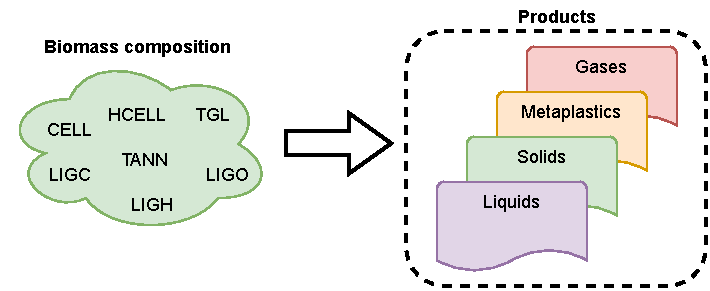
\includegraphics[width=0.7\textwidth]{figures/biocomp1.pdf}
    \caption{Seven biomass components convert to pyrolysis products according to the Debiagi et al. biomass pyrolysis kinetics scheme.}
    \label{fig:biocomp1}
\end{figure}

\subsection{Biomass composition}

According to the Debiagi et al. 2015 paper \cite{Debiagi-2015}, the chemical components of the biomass are defined as shown in Table \ref{tab:chem-components}. The Debiagi paper does not provide information on how to experimentally determine these components. However, the paper provides a characterization method which estimates the biomass composition based on elemental (ultimate) analysis data. The characterization method uses the carbon (C) and hydrogen (H) content of the biomass to predict the biochemical composition in terms of cellulose, hemicellulose, lignin, tannins, and triglycerides. Splitting parameters $\alpha$, $\beta$, $\gamma$, $\delta$, and $\epsilon$ are used to improve the validity of the characterization procedure by accounting for extractives in the biomass.

\begin{table}[H]
    \centering
    \caption{Chemical components representing biomass composition needed for the Debiagi et al. pyrolysis kinetics.}
    \label{tab:chem-components}
    \begin{tabular}{lp{2cm}p{7cm}}
        \toprule
        Biomass composition & Symbol & Description \\
        \midrule
        cellulose     & CELL & glucan \\
        \addlinespace[0.2in]
        hemicellulose & GMSW XYHW XYGR & mixture of sugars such as hexoses and pentoses; mainly xylose, mannose, galactose, and arabinose \\
        \addlinespace[0.2in]
        lignin        & LIG & aromatic alcohols such as coniferyl, sinapyl, p-coumaryl alcohol\\
        \addlinespace[0.2in]
        lignin-c      & LIG-C & carbon-rich lignin \\
        \addlinespace[0.2in]
        lignin-h      & LIG-H & hydrogen-rich lignin \\
        \addlinespace[0.2in]
        lignin-o      & LIG-O & oxygen-rich lignin \\
        \addlinespace[0.2in]
        tannins       & TANN & hydrophilic extractives, phenolics, ethanol and water, represented by a gallocatechin polymer \\
        \addlinespace[0.2in]
        triglycerides & TGL & hydrophobic extractives, hexane and ether, linoleic acid \\
        \bottomrule
    \end{tabular}
\end{table}

As discussed previously, the largest differences in the chemical analysis feedstock data are for the lignin, glucan, and mannan fractions. These fractions represent the cellulose (glucan), hemicellulose (xylan, galactan, arabinan, mannan, acetyl), and total lignin components of the biomass composition. Unfortunately, the chemical analysis data does not directly relate to all the biomass compositional components needed for the pyrolysis kinetics.

Using the C and H values from the ultimate analysis CHO basis and default values for the splitting parameters, the biomass composition is estimated using the characterization method from Debiagi et al. The estimated cellulose, hemicellulose, and total lignin (LIGC + LIGH + LIGO) values are compared to the chemical analysis measurements using

\begin{equation}
    f(\alpha, \beta, \gamma, \delta, \epsilon) = (cell_{est} - cell_{meas})^2 + (hemi_{est} - hemi_{meas})^2 + (lignin_{est} - lignin_{meas})^2
\end{equation}

\noindent where $f$ is the function to be minimized, $cell_{est}$ is the estimated cellulose, $cell_{meas}$ is the cellulose from chemical analysis, $hemi_{est}$ is the estimated hemicellulose, $hemi_{meas}$ is the hemicellulose from chemical analysis, $lignin_{est}$ is the estimated lignin, and $lignin_{meas}$ is the lignin from chemical analysis. The L-BFGS-B algorithm is applied to the minimization function to generate the optimum splitting parameter values such that the estimated cellulose, hemicellulose, and total lignin are similar to the values obtained from the chemical analysis data. Figure \ref{fig:biocomp2} demonstrates the biomass composition minimization procedure.

\begin{figure}[H]
    \centering
    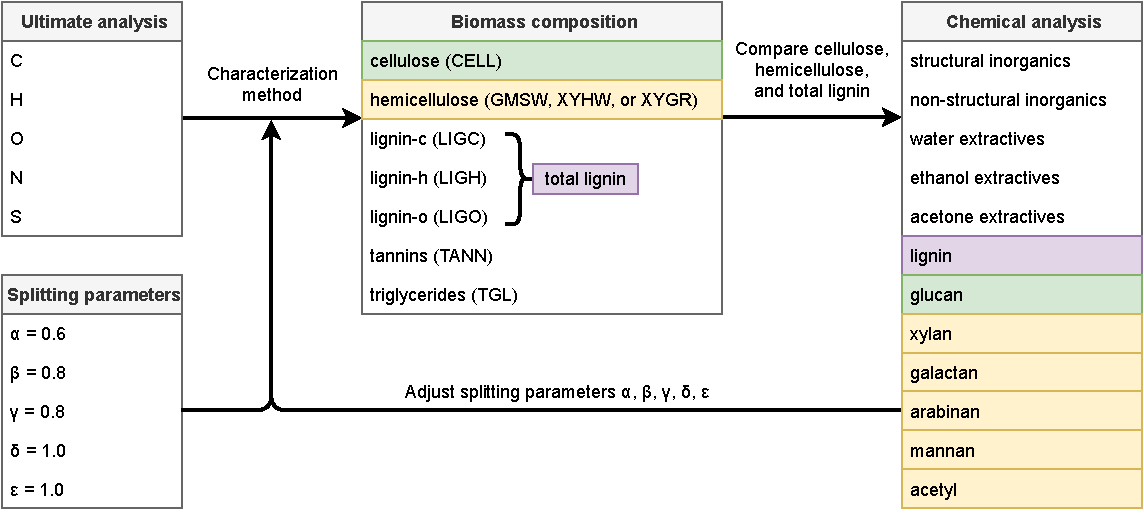
\includegraphics[width=\textwidth]{figures/biocomp2.pdf}
    \caption{Biomass composition determined from ultimate analysis data and compared with measured chemical analysis data for cellulose, hemicellulose, and total lignin.}
    \label{fig:biocomp2}
\end{figure}

\subsection{Batch reactor and CSTR models}

The material balance for a chemical reactor considers the inlet and outlet flows of the system along with accumulation and reaction effects

\begin{equation}
    \begin{aligned}
        accumulation &= input - output + reaction \\
        \frac{dC_A}{dt} V &= v C_{A0} - v C_A + r_A V
    \end{aligned}
\end{equation}

\noindent where $A$ represents some chemical species, $C_A$ is the outlet concentration (mol/m$^3$), $C_{A0}$ is the inlet concentration (mol/m$^3$), $V$ is the reactor volume (m$^3$), $v$ is the volumetric flow rate (m$^3$/s), and $r_A$ is the reaction rate (mol/m$^3$s). The reaction rate is determined by multiplying a forward rate constant $k$ by the concentration in the tank. The rate constant is calculated from an Arrhenius function

\begin{equation}
    \label{eq:rate-constant}
    k = A\,T^b e^{-E / RT}
\end{equation}

\noindent where $A$ is the pre-exponential factor, $T$ is the reaction temperature, $b$ is the temperature exponent, $E$ is the activation energy, and $R$ is the universal gas constant.

A batch reactor is modeled to understand the time scales associated with the biomass pyrolysis kinetics. For a batch reactor, input and output is zero therefore only the accumulation and reaction terms remain in the material balance. For a constant volume reactor the $V$ terms cancel out resulting in the following material balance for a batch reactor model

\begin{equation}
    \label{eq:batch-balance}
    \begin{aligned}
        accumulation &= 0 - 0 + reaction \\
        \frac{dC_A}{dt} &= r_A
    \end{aligned}
\end{equation}

\noindent A depiction of a batch reactor is shown in Figure \ref{fig:batch-cstr}. The Cantera Python package is used to model the batch reactor as an IdealGasReactor object \cite{Cantera-2018}.

\begin{figure}[H]
    \centering
    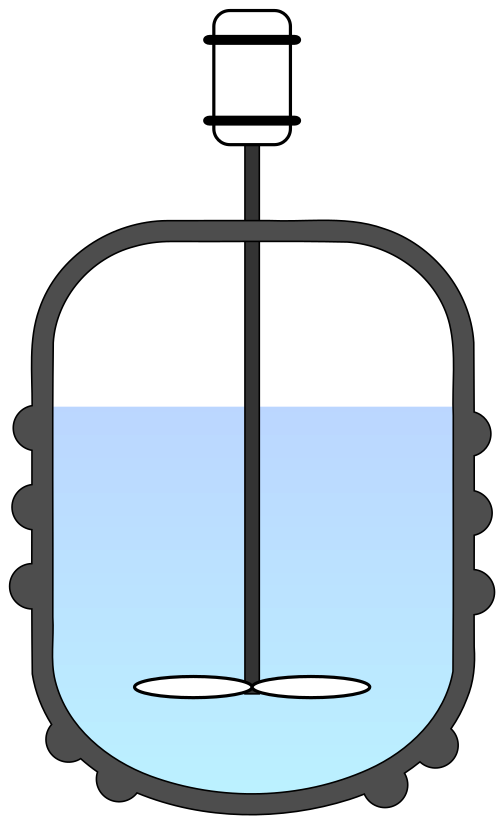
\includegraphics[width=0.2\textwidth]{figures/reactor-batch.png}
    \hspace{0.1\textwidth}
    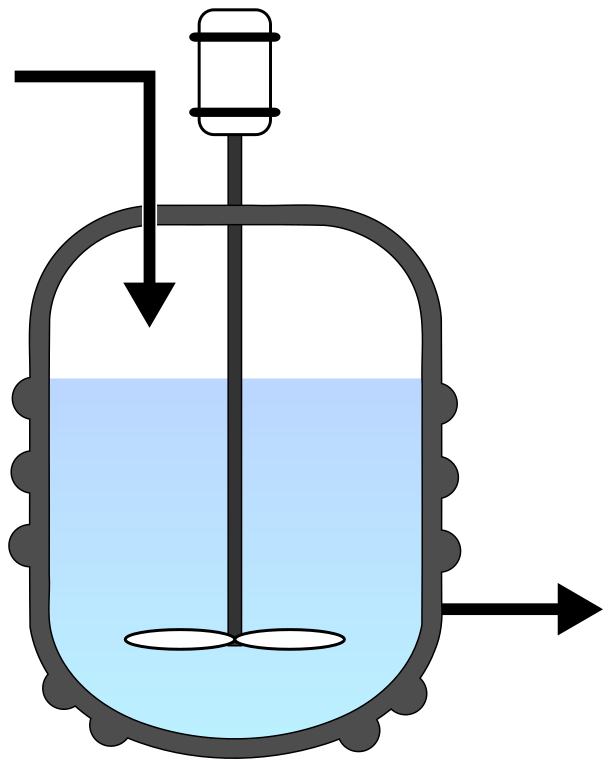
\includegraphics[width=0.265\textwidth]{figures/reactor-cstr.png}
    \caption{Representation of a batch reactor (left) and a continuous stirred-tank reactor (right). Source: Wikipedia.}
    \label{fig:batch-cstr}
\end{figure}

To account for inlet and outlet flows, residence time, and reactor geometry, a continuous stirred tank reactor (CSTR) system at steady-state conditions is also modeled. The material balance for a steady-state CSTR does not account for accumulation but does consider the residence time in the system

\begin{equation}
    \begin{aligned}
        0 &= input - output + reaction \\
        0 &= v C_{A0} - v C_A + r_A V \\
        C_A &= C_{A0} + r_A\;\tau \\
    \end{aligned}
\end{equation}

\noindent where $\tau$ is the residence time (s) of chemical $A$ in the reactor. A depiction of a CSTR system with its inlet and outlet flows is shown in Figure \ref{fig:batch-cstr}. The Cantera Python package is used to model the CSTR using an IdealGasReactor object with inlet and outlet flows \cite{Cantera-2018}.

A series of CSTRs are modeled to represent the mixing (residence time) of the different feedstocks in the NREL fluidized bed reactor. The average residence time for each feedstock is obtained from CFD simulations performed by NETL. As the number of CSTRs increases, the reactor model behaves more like a plug flow reactor (PFR). This modeling technique is illustrated by Figure \ref{fig:reactor-cstr-series} where the subscript $n$ represents the total number of CSTRs. The residence time $\tau$ in each CSTR is calculated as

\begin{equation}
    \tau = \frac{\tau_{avg}}{n}
\end{equation}

\noindent where $\tau_{avg}$ is the average residence time from CFD simulations and $n$ is the total number of CSTRs in series.

\begin{figure}[H]
    \centering
    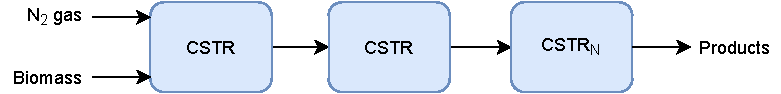
\includegraphics[width=0.8\textwidth]{figures/reactor-cstr-series.pdf}
    \caption{Depiction of a bubbling fluidized bed reactor modeled as a series of CSTRs.}
    \label{fig:reactor-cstr-series}
\end{figure}

To exclude the nitrogen gas fraction from the calculated CSTR product yields, the mass fractions are converted from a N$_2$ basis to a N$_2$ free basis

\begin{equation}
    Y_{i,\,N_2\,free} = \frac{Y_{i,\,N_2}}{Y_{gas,\,N_2} + Y_{liquid,\,N_2} + Y_{solid,\,N_2} + Y_{metaplastic,\,N_2} - Y_{N_2}}
\end{equation}

\noindent where $Y$ is the mass fraction and the subscript $i$ represents the gas, liquid, solid, and metaplastic phases.
